%auto-ignore
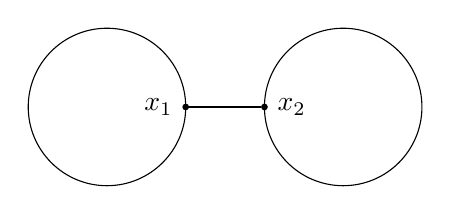
\begin{tikzpicture}
 \tikzset{point/.style = {draw, circle, fill=black, minimum size=2pt,inner sep=0pt}}
 \tikzset{->-/.style={decoration={markings,mark=at position #1 with {\arrow{>}}},postaction={decorate}}}
 \def\rad{1cm}
 \def\len{3cm}
 
 \node (C1) at (0,0) {};
 \node (C2) at (\len,0) {};
 \draw (C1) circle (\rad);
 \draw (C2) circle (\rad);
 
 \path (C1) node[point,label={180:$x_1$}] (x1)  at +(0:\rad) {};
 \path (C2) node[point,label={0:$x_2$}] (x2)  at +(180:\rad) {};
 
 \draw (x1) -- (x2);
  
\end{tikzpicture}
